%\documentclass[conference,spanish,a4paper,10pt,oneside,final]{IEEEtran}
\nonstopmode
\documentclass[conference,spanish,a4paper,10pt,oneside,final]{tfmpd}

\include{conf/preconfig}
\include{conf/packages}
%
% Propiedades del documento: título, autor, etc
%
%% \newcommand{\titulo}{{\large FICH --- UNL}\\Procesamiento Digital de Imágenes
%% 2010\\Trabajo Final}
%% \newcommand{\autor}{Fornal, Esteban \and Pfarher, Christian \and Torrez, Mauro}
%% \newcommand{\fecha}{\today}
%% \newcommand{\tituloPDF}{Trabajo Final PDI 2010}
%% \newcommand{\autorPDF}{Fornal, Pfarher, Torrez}
%% \newcommand{\asuntoPDF}{}
%% \newcommand{\clavesPDF}{}
%
\include{conf/config}
%\include{conf/comandos}
%
\begin{document}
\title{Identificación de edificios y monumentos a partir de fotografías
tomadas con dispositivos móviles}
\author{Esteban C. Fornal, Christian N. Pfarher, Mauro J. Torrez\\
\textit{Trabajo práctico final de ``Procesamiento Digital de
Imágenes'', II-FICH-UNL.}}
\markboth{Procesamiento Digital de Imágenes: TRABAJO FINAL}{}
\maketitle
%
%
% %%%%%%%%%%%%%%%%%%%%%%%%%%%%%%%%%%%%%%%%%%%%%%%%%%%%%%%%%%%%%%%%%%%%%%%%%%%%%%
%
%
\begin{abstract}
%% El objetivo de este trabajo consiste en la identificación de edificios y
%% monumentos, a partir de imágenes obtenidas mediante un dispositivo móvil de
%% características estándar en el mercado. Para dicho propósito se plantearán
%% métodos diferentes, uno mediante extracción de características en el espacio
%% de la Transformada de Hough y otro basado en medidas estadísticas, comparando
%% a cada uno de ellos por separado y finalmente, evaluando el desempeño de la
%% utilización de ambos conjuntamente.
Se presenta un método para la identificación de edificios y monumentos, a
partir de fotografías tomadas con la cámara de un dispositivo móvil.
Para la identificación se extrae un vector de características de la imagen,
que es almacenado en una base de datos para su consulta.
Se presentan dos métodos para la extracción de características en la imagen, uno
basado en la transformada de Hough y otro que utiliza estadísticas de los
histogramas. Se evalúa el desempeño utilizando ambos métodos por separado y en
conjunto, para una base de datos de prueba de unas pocas imágenes.
\end{abstract}
%
%
% %%%%%%%%%%%%%%%%%%%%%%%%%%%%%%%%%%%%%%%%%%%%%%%%%%%%%%%%%%%%%%%%%%%%%%%%%%%%%%
%
%
\begin{keywords}
Identificación/reconocimiento de edificios, \eng{building recognition},
histograma, extracción de características, transformada de Hough, clasificación.
\end{keywords}
%
%
% %%%%%%%%%%%%%%%%%%%%%%%%%%%%%%%%%%%%%%%%%%%%%%%%%%%%%%%%%%%%%%%%%%%%%%%%%%%%%%
%
%
\section{Introducción}
\PARstart{L}{a} presencia de gran cantidad de dispositivos tecnológicos de
diferente índole ha abierto un sin número de nuevas aplicaciones para
satisfacer las necesidades diarias de seres humanos. Los dispositivos móviles
como celulares, PDAs, etc. han pasado a formar parte del común de nuestras
vidas brindando nuevas posibilidades de interacción. Es aquí donde surge la
idea de la realización de este trabajo. 

Día a día, las personas toman fotografías de diferentes objetos ya sean
monumentos públicos, edificios históricos, etc. sin saber si quiera que se
está fotografiando. Con este artículo se trata de hacer un aporte en vías
hacia dicho problema, de manera que mediante el procesamiento de imágenes se
tenga dicha información en el instante mismo de la adquisición de la foto.
Cabe aclarar, que se hará una implementación en C++, dejando como trabajo
futuro el desarrollo de una aplicación para dispositivos móviles.

En principio y ya que no es el objetivo de este trabajo hacer un análisis
profundo, sino tan solo dar una aproximación inicial a la resolución del
problema, se considerará la aplicación de los métodos en condiciones
ideales o semi-ideales. \resalt{ver...}
%
%
% %%%%%%%%%%%%%%%%%%%%%%%%%%%%%%%%%%%%%%%%%%%%%%%%%%%%%%%%%%%%%%%%%%%%%%%%%%%%%%
%
%
\section{Método propuesto}
El método que proponemos se basa en la extracción de características de la
imagen y la comparación de éstas con las de una base de datos.
Esta base de datos se genera tomando $X$ imágenes representativas del monumento,
extrayendo sus características y promediándolas para obtener un prototipo
``generalizado'' del monumento/edificio a detectar.

La extracción de características se realiza en este trabajo mediante dos
técnicas diferentes:
\begin{enumerate}
\item extracción de características por transformada de Hough, y
\item extracción de características por estadísticas del histograma.
\end{enumerate}

El entrenamiento de la base de datos se realiza obteniendo las características
para cada imagen, junto con su etiqueta. Para cada etiqueta, se extraen las
características de las $X$ imágenes etiquetadas con la misma, y se guarda un
``prototipo'' obtenido de promediar estas características, junto con la
etiqueta.

La clasificación de las imágenes consiste en encontrar la etiqueta del
prototipo cuyas características minimicen el error cuadrático medio.
%
%%%%%%%%%%%%%%%%%%%%%%%%%%%%%%%%%%%%%%%%%%%%%%%%%%%%%%%%%%%%%%%%%%%%%%%%%%%%%%%%
%
\subsection*{Extracción de características mediante Transformada de Hough}
La transformada de Hough nos permite visualizar, a partir de una imagen de
bordes, los parámetros de aquellas rectas\footnote{El procedimiento es general,
sirve para cualquier geometría que se pueda expresar en términos de sus
parámetros. En este trabajo, utilizamos el espacio de los parámetros de las
rectas, el más sencillo.}
que son principales en la imagen.

Para la extracción de características con esta técnica se siguen los siguientes
pasos:
\begin{enumerate}
\item A partir de la imagen original, se obtiene una versión en escala de grises
      promediando los tres canales RGB, y se la escala a un tamaño normalizado.
\item Se obtiene una imagen de sólo bordes, aproximando la magnitud del
      gradiente según
      \begin{equation}
      \label{sob}
      \nabla f \approx |G_x| + |G_y|,
      \end{equation}
      donde $G_x$, $G_y$ son el resultado de aplicar los operadores gradiente
      de Sobel (fig. \ref{masksobel}) a la imagen. 
      Finalmente se umbraliza esta imagen de bordes en $U$:
      \begin{equation}
      \label{umbral}
      f(x)=
      \begin{cases}
      0, & x\leq U\\
      255, & x > U
      \end{cases}
      \end{equation}
\item Con la imagen de bordes umbralizada se calcula la transformada de
      Hough para rectas.
\item Se aplica escalado a la transformada obtenida, llevándola a un tamaño
      pequeño buscando obtener mayor tolerancia tanto en el parámetro angular
      $\theta$ como de distancia $\rho$
\item Se toman $N$ máximos de esta transformada y se guardan en el vector de
      características las coordenadas $(\rho,\theta)$, mapeadas al rango
      $[-1,1]$ obteniendo así un vector de $2N$ valores.
\end{enumerate}
%% Como se puede observar en la Fig. \ref{procesohough}, en el primer paso se
%% obtiene una imagen de un solo canal mediante el promediado de los tres
%% canales RGB. Luego, con el objetivo de disminuir el costo computacional, se
%% realiza un redimensionamiento de la imagen de 640 x 480 pixels a 100x100.
%% Posteriormente, para la detección de bordes se aplica el operador gradiente
%% de sobel (\ref{sob}) y se umbraliza con la función definida en
%% (\ref{umbral}).
\begin{figure}
\begin{center}
\begin{tabular}{|c|c|c|}
\hline -1 & -2 & -1 \\\hline 0 & 0 & 0 \\\hline 1 & 2 & 1 \\\hline
\end{tabular}
\begin{tabular}{|c|c|c|}
\hline -1 & 0 & 1 \\\hline -2 & 0 & 2 \\\hline -1 & 0 & 1 \\\hline
\end{tabular}
\end{center}
\caption{Máscaras de filtrado (operadores gradiente) de Sobel.}
\label{masksobel}
\end{figure}


%

%
%
%% Tras estos pasos, se transforma al espacio de Hough y aquí se aplica nuevamente un redimensionado a tamaño de 40x40 con el fin de tener una tolerancia respecto a $\rho$ y $\theta$ del espacio transformado de Hough.\resalt{no me gusta arreglar}
%% Finalmente, se obtienen las coordenadas $\rho$ y $\theta$ de 50 máximos con las cuales se forma el vector de características representativo de la imagen.
\begin{figure}
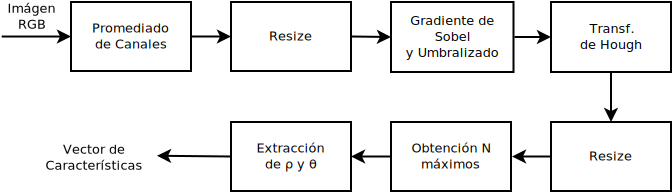
\includegraphics[scale=0.25]{../diagramas/procesohough} 
\caption{"Proceso de la imagen mediante el método por T. de Hough"}
\label{procesohough}
\end{figure}
%
%%%%%%%%%%%%%%%%%%%%%%%%%%%%%%%%%%%%%%%%%%%%%%%%%%%%%%%%%%%%%%%%%%%%%%%%%%%%%%%%
%
\subsection*{Extracción de características por estadísticas del histograma}
A partir de la imagen original, se normaliza su tamaño y se toman 2 ``perfiles de
intensidad'': uno horizontal, calculado promediando cada columna de la imagen, y
otro vertical obtenido al promediar cada fila. Se obtiene un histograma para la
imagen entera y uno para cada perfil, y se guardan en el vector de
características la media aritmética $m$, mediana $M$ (posición del percentil 50),
 y desviación absoluta $D_{\T{abs}}$ respecto de la mediana:
\begin{equation*}
D_{\T{abs}}=\sum_i |x_i - M|
\end{equation*}
Así se han obtenido un vector de 9 valores que caracterizan histogramas de la
imagen entera.

Luego se subdivide la imagen en cuatro cuadrantes, y se obtienen para cada uno
las mismas medidas que se calcularon para la imagen entera.

Así se obtiene un vector de 45 características a partir de histogramas que se
guardarán en la base de datos para comparación.

\begin{figure}
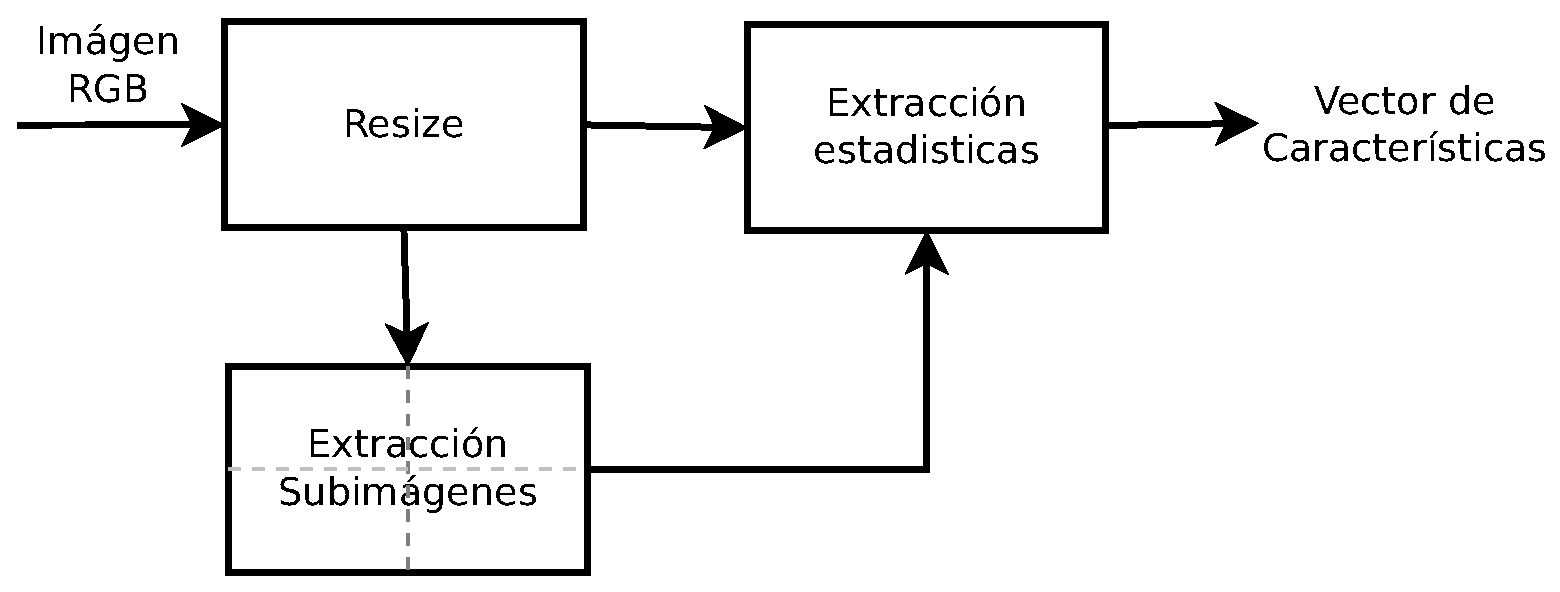
\includegraphics[scale=0.25]{../diagramas/procesoestadisticas} 
\caption{"Proceso de la imagen mediante el método de estadísticas del histograma"}
\label{procesohough}
\end{figure}

%
%%%%%%%%%%%%%%%%%%%%%%%%%%%%%%%%%%%%%%%%%%%%%%%%%%%%%%%%%%%%%%%%%%%%%%%%%%%%%%%%
%
\subsection*{}

%
%
%%%%%%%%%%%%%%%%%%%%%%%%%%%%%%%%%%%%%%%%%%%%%%%%%%%%%%%%%%%%%%%%%%%%%%%%%%%%%%%%
%
%
\section{Experimentos y resultados}
Para las pruebas se procedió a evaluar el desempeño de ambos métodos, en primera instancia por separados y luego, conjuntamente.
%
%%%%%%%%%%%%%%%%%%%%%%%%%%%%%%%%%%%%%%%%%%%%%%%%%%%%%%%%%%%%%%%%%%%%%%%%%%%%%%%%
%
\subsection{Descripción de la Base de datos de imágenes}
Se trabajó con imágenes que fueron adquiridas en la ciudad de Santa Fe, mediante un Dispositivo Móvil con una resolución de 640x480 pixels. Se construyo una base de datos de las mismas sobre un total de cinco edificios, tomando trece realizaciones de cada uno de ellos (diez con el propósito de usarlas como prototipo y tres para las prueba con los algoritmos). Cabe aclarar que cada conjunto de imágenes de los cinco edificios fueron tomadas en condiciones ambientales similares y con la cámara en la misma posición respecto del objetivo. \resalt{arreglar esto}.
%%%%%%%%%%%%%%%%%%%%%%%%%%%%%%%%%%%%%%%%%%%%%%%%%%%%%%%%%%%%%%%%%%%%%%%%%%%%%%%%%%
\subsection{Vectores característicos y prototipos}
Sobre diez de las trece imágenes de cada edificio, se aplicó el método de al Transformada de Hough citado en este artículo, obteniéndose diez vectores representativos (uno por cada imagen) y se procedió a promediar dichos vectores dando como resultado un prototipo por cada edifico. De la misma manera se realizó el mismo proceso, con el método estadístico descripto también en este documento.
%%%%%%%%%%%%%%%%%%%%%%%%%%%%%%%%%%%%%%%%%%%%%%%%%%%%%%%%%%%%%%%%%%%%%%%%%%%%%%%%%%

\subsection{Descripción de las pruebas}
Por cada método se calculo el MSE o error cuadrático medio definido en \ref{mse} entre los cinco prototipos y las quince imágenes de pruebas, para finalmente obtener la tasa de reconocimiento mediante \ref{tasareconocimiento}
\begin{equation}
MSE=\ldots \label{mse}
\end{equation}
\begin{equation}
\% reconocimiento = \frac{\# aciertos}{15} \label{tasareconocimiento}
\end{equation}
%
%
% %%%%%%%%%%%%%%%%%%%%%%%%%%%%%%%%%%%%%%%%%%%%%%%%%%%%%%%%%%%%%%%%%%%%%%%%%%%%%%
%
%
\subsection{Tablas}
\begin{tabular}{cc}
\hline columna1 & columna2 \\ 
\hline  &  \\ 
\hline 
\end{tabular} 
%
%
% %%%%%%%%%%%%%%%%%%%%%%%%%%%%%%%%%%%%%%%%%%%%%%%%%%%%%%%%%%%%%%%%%%%%%%%%%%%%%%
%
%
\subsection{Discusión}
blablabla
%
%
% %%%%%%%%%%%%%%%%%%%%%%%%%%%%%%%%%%%%%%%%%%%%%%%%%%%%%%%%%%%%%%%%%%%%%%%%%%%%%%
%
%
\section{Conclusiones}
blablabla
%
%
% %%%%%%%%%%%%%%%%%%%%%%%%%%%%%%%%%%%%%%%%%%%%%%%%%%%%%%%%%%%%%%%%%%%%%%%%%%%%%%
%
%
\section{Trabajos futuros}
A partir del diseño aquí presentado, seguiremos investigando esta técnica con las siguientes
posibilidades:
\begin{itemize}
\item Considerar la aplicación de un filtrado homomórfico en imágenes que lo requieran.
\item Independizarse de la posición en que se tomó la fotografía con alguna técnica de warping.
\item Arreglar el metodo de Hough que es una X onga jaja\end{itemize}

\nocite{*}
\bibliographystyle{tfmpd}
\bibliography{tfmpd}
\end{document}

